\chapter{Results and Conclusion} \label{ch:cando}

Up to this point I have given an overview of the physics background for jets created in high energy particle collisions, a description of the ALICE detector, and the steps needed to prepare the data for an analysis.  The final portion of this thesis will combine all of the results and corrections together in order to present the final cross sections.  However, in order to present the final cross-section we will need to discuss the systematic errors that contribute to the final uncertainty in my reported results.

\section{Systematic Uncertainties}

Systematic uncertainties arise due to our limited knowledge of the precise operating conditions and performance of the experiment, they also are due to any bias in our understanding of how to fundamentally model the interactions.  The systematics may be broken into two categories: uncertainties to the jet energy scale (JES) which shifts the momentum spectra along the momentum axis, and uncertainties in the jet yield, which shift the spectra along the spectra/cross-section axis.  The systematical and statistical uncertainties presented in this analysis will be presented as errors to the yield of the spectra.  Due to the fact that the $p_{T}$ distribution follows a power law function, $d\sigma/dp_{T} \sim p_{T}^{-5}$ uncertainties to the JES are converted to yield uncertainties by dividing each one by five.
The low statistics at the highest $p_{T}$ bins in this analysis mean that uncertainties in this range may have large statistical fluctuations.  Another way to put this is that small systematic variations for the input of the jet spectra will have a dramatic effect over sparsely filled bins versus bins with a low granularity.  As such it may be necessary to extrapolate the systematic from a low $p_{T}$ bin to those at the highest $p_{T}$ range.  The systematics were performed on both the Min Bias and EMCal triggered data samples but no large variation was observed between the two, thus only the uncertainties from the Min Bias sample are shown and are extrapolated to the triggered data.


\subsection{Systematic Uncertainty to Jet Energy Scale}

The following sections present and discuss the uncertainties caused by shifts to the JES.  These uncertainties were divided by a factor of 5 to convert to uncertainties on the y-axis which reports jet cross-sections.

\subsubsection{Tracking Efficiency Sensitivity}
Only a fraction of charged tracks generated by the hard scattering of two protons will be detected in the TPC due to its finite track efficiency.  Uncertainties in the efficiency of the TPC were studied and found to account for a 5\% discrepancy\cite{Abelev:2013ala} between the number of tracks in a collision versus the number of measured tracks in proton-proton collisions.  In order to obtain the error associated with this efficiency, this analysis was reperformed maintaining all the cuts and QA discussed in Chapter \ref{ch:analysis}, while throwing out 5\% of the tracks from each event and remeasuring the jet spectra.  Once this new jet spectra was generated, it was corrected using the bin-by-bin corrections and the ratio of this new spectra was taken with the original spectra to gauge the uncertainty from the tracking efficiency.


\begin{figure*}[t!]
$\begin{array}{rl}
    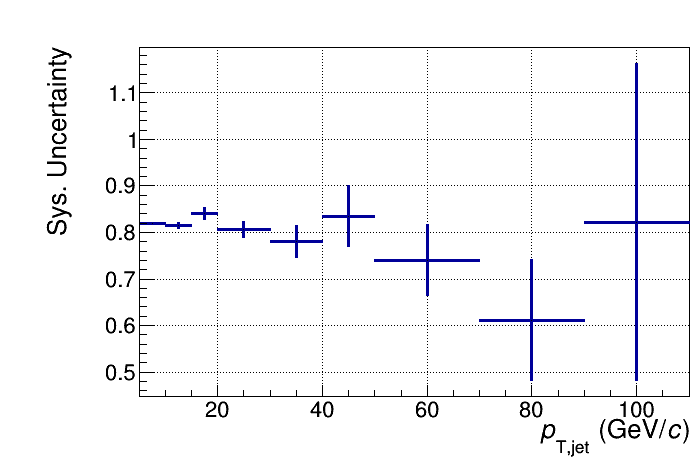
\includegraphics[width=0.40\textwidth]{SysR02_TrkEff} &
    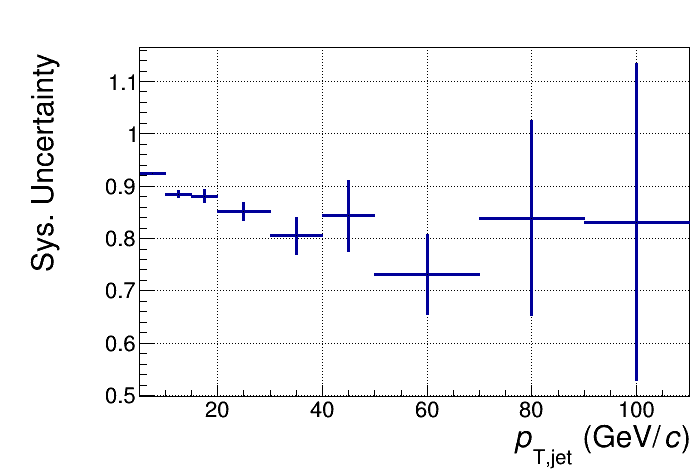
\includegraphics[width=0.40\textwidth]{SysR03_TrkEff}\\
    \multicolumn{2}{c}{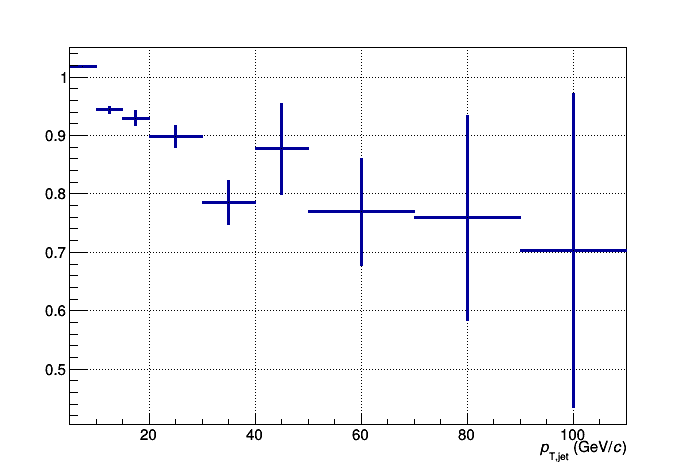
\includegraphics[width=0.40\textwidth]{SysR04_TrkEff}}
\end{array}$
\caption[Systematic due to TPC tracking efficiency.]{\label{fig:trkeff}Systematic due to TPC tracking efficiency; R = 0.2 \textit{(top left)}, R = 0.3 \textit{(top right)}, R = 0.4 \textit{(bottom)}.}
\end{figure*}

\noindent
Figure \ref{fig:trkeff} shows the systematical uncertainties for R = 0.2, R = 0.3, and R = 0.4 jets.  From the figures a 10\% systematic was assigned to R = 0.2 and R = 0.3 jets, while a 15\% systematic uncertainty was given to R = 0.4 jets for this analysis.

\subsubsection{Hadronic Correction}

\begin{figure*}[t!]
$\begin{array}{rl}
    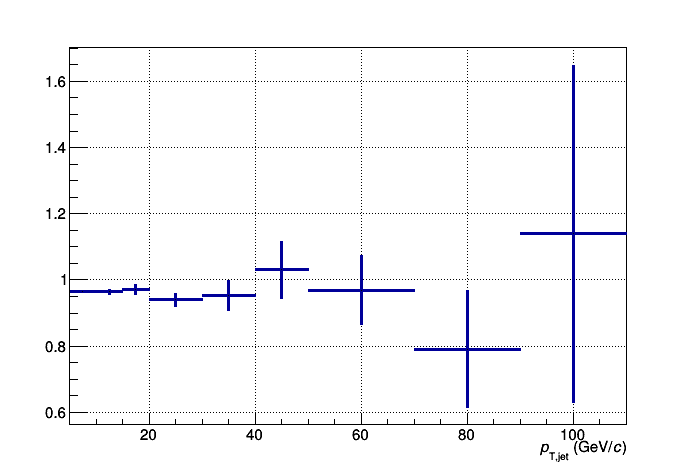
\includegraphics[width=0.40\textwidth]{SysR02_F07} &
    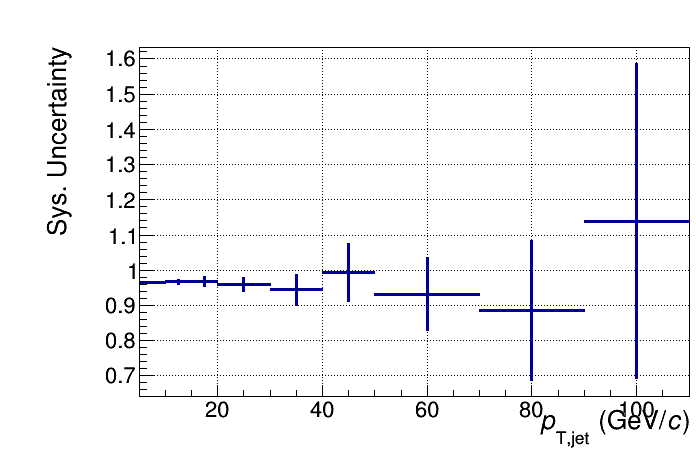
\includegraphics[width=0.40\textwidth]{SysR03_F07}\\
    \multicolumn{2}{c}{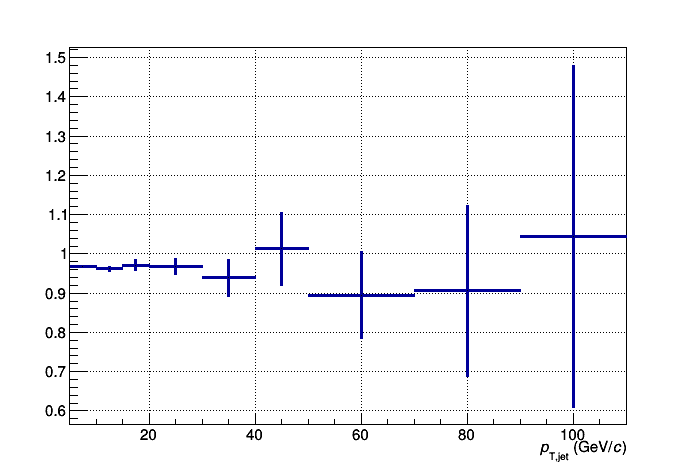
\includegraphics[width=0.40\textwidth]{SysR04_F07}}
\end{array}$
\caption[Systematic due to Hadronic correction.]{\label{fig:hadeff}Systematic due to hadronic correction efficiency; R = 0.2 \textit{(top left)}, R = 0.3 \textit{(top right)}, R = 0.4 \textit{(bottom)}.}
\end{figure*}

In order to assign an uncertainty to the hadronic correction applied to EMCal clusters, the nominal value of $f_{sub} = 1$ in equation \ref{eq:HadCorr} was changed to a value of 0.7 and the analysis chain is repeated.  Figure \ref{fig:hadeff} shows the ratio of the new spectra with the original, and the uncertainty due to the hadronic correction was around 5\% for all jet radii.

\subsubsection{Sensativity to EMCal Clusterization Algorithm}
As previously stated, the clusterizer used in this thesis was the v2 algorithm, which limits the number of EMCal towers in a cluster to a maximum of nine. This algorithm was used in both the detector-level Monte Carlo and data analysis.  In order to test the sensitivity the JES has to the clusterization algorithm, a different algorithm was chosen and a new spectra was generated.  The v1 algorithm was chosen and is similar to the v2 algorithm with the exception that the total size of the cluster is forced to be smaller then nine towers .  Similar to the other systematics presented, we see large anti-correlated variations at high-$p_{T}$ due to sparsely field binning.  

\begin{figure*}[t!]
$\begin{array}{rl}
    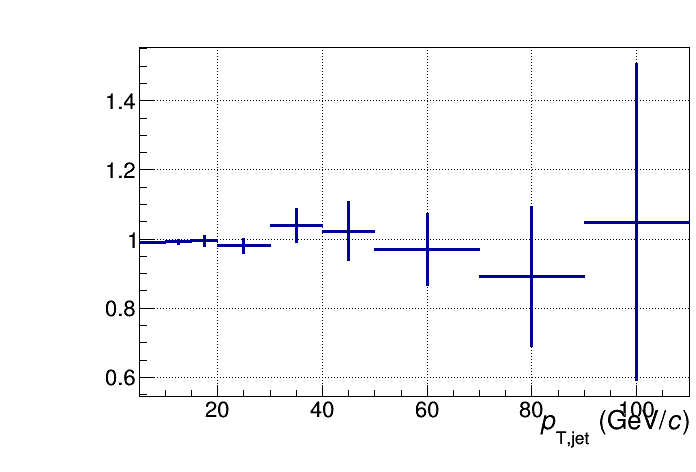
\includegraphics[width=0.40\textwidth]{SysR02_v1Clusterization} &
    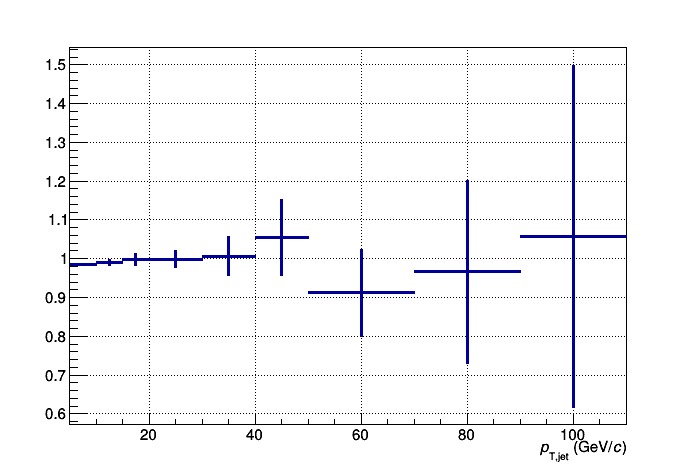
\includegraphics[width=0.40\textwidth]{SysR03_v1Clusterization}\\
    \multicolumn{2}{c}{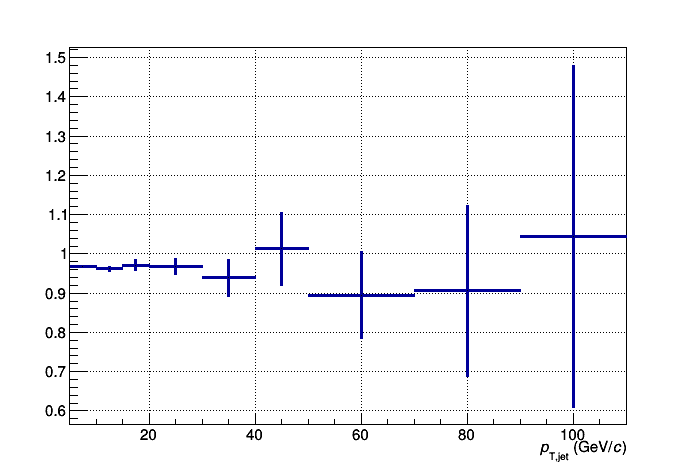
\includegraphics[width=0.40\textwidth]{SysR04_F07}}
\end{array}$
\caption[Systematic due to clusterization algorithm.]{\label{fig:cluseff}Systematic due to EMCal clusterization algorithm; R = 0.2 \textit{(top left)}, R = 0.3 \textit{(top right)}, R = 0.4 \textit{(bottom)}.}
\end{figure*}

Figure \ref{fig:cluseff} shows the systematic uncertainty to the clusterization for each of the jet radii.  At low-$p_{T}$ I assigned an uncertainty of between 1\% and 3\% for a given jet radii.  At high-$p_{T}$ I assigned a 5\% for R = 0.2 and 10\% uncertainty for R = 0.3 and R=0.4 jets to help account for the statistical fluctuations.

\subsection{Systematic Uncertainty to Jet Yield}

The following sections discuss the systematic uncertainties affecting the jet yield.

\subsubsection{Track $p_{T}$ Resolution}

\begin{figure}[h]
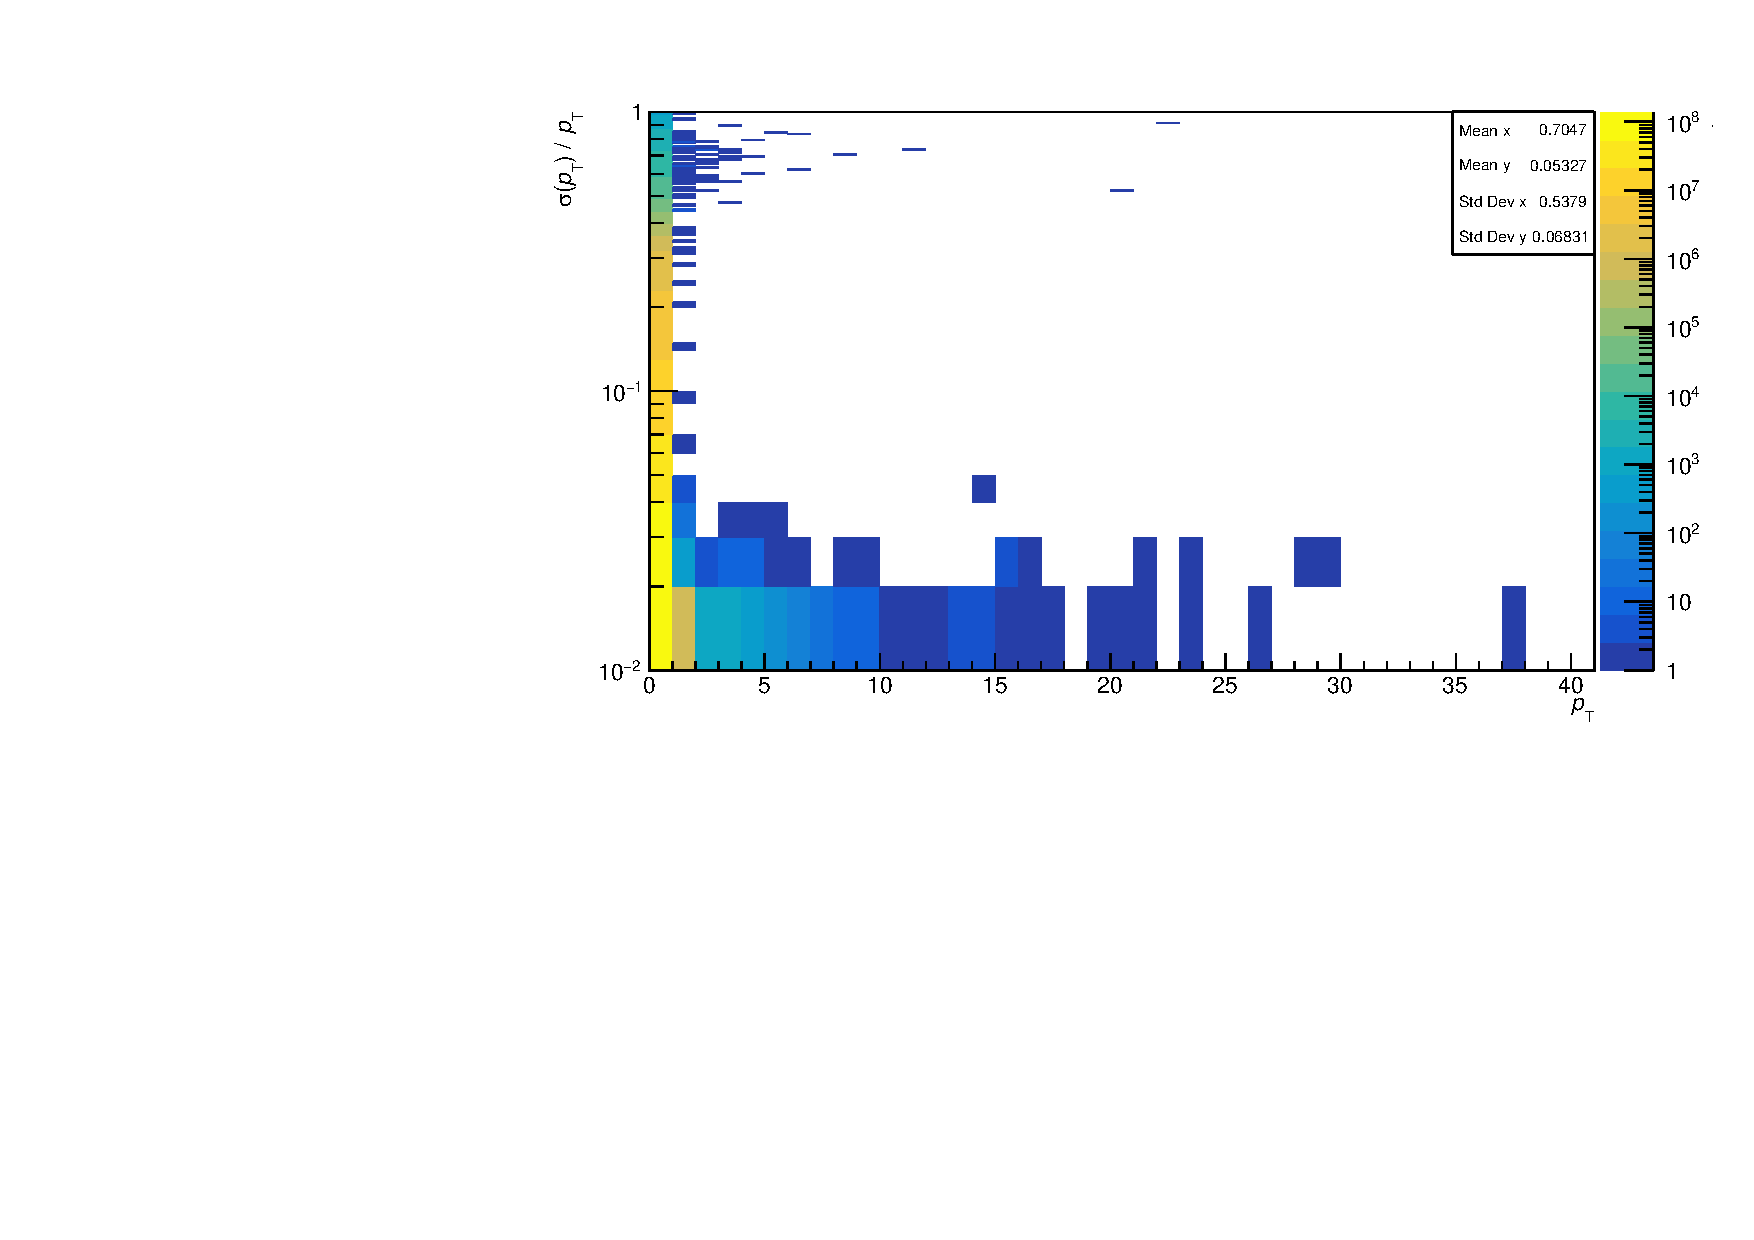
\includegraphics[width=8cm]{trackcovmatrix}
\centering
\caption{Inclusive track resolution, Min Bias 8 TeV.}
\label{fig:trackpcovmatrix}
\end{figure}

\begin{figure*}[t!]
$\begin{array}{rl}
    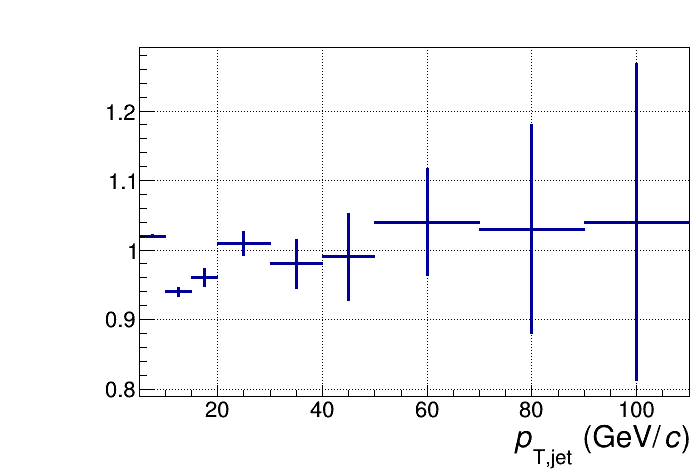
\includegraphics[width=0.40\textwidth]{SysR02_PtReso} &
    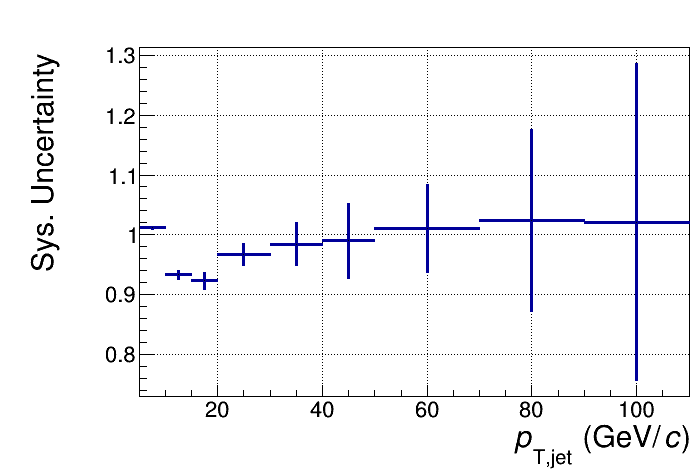
\includegraphics[width=0.40\textwidth]{SysR03_PtReso}\\
    \multicolumn{2}{c}{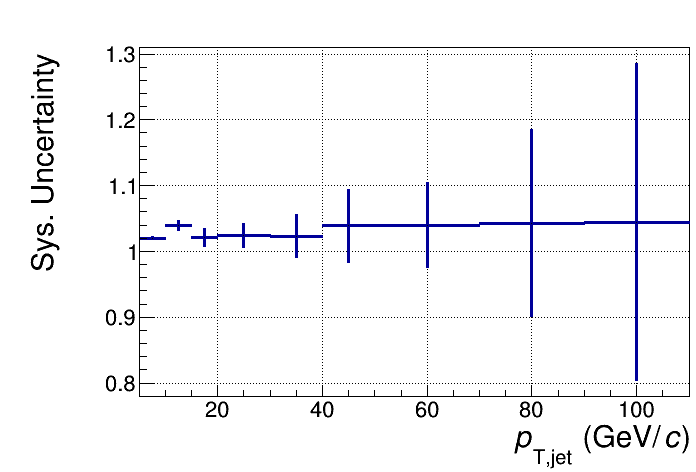
\includegraphics[width=0.40\textwidth]{SysR04_PtReso}}
\end{array}$
\caption[Systematic due to $P_{T}$ resolution.]{\label{fig:pTeff}$P_{T}$ resolution systematic; R = 0.2 \textit{(top left)}, R = 0.3 \textit{(top right)}, R = 0.4 \textit{(bottom)}.}
\end{figure*}

\noindent
The momentum resolution of TPC is estimated using the covariance matrix generated from the Kalman filtering\cite{Fruhwirth:1987fm} pad signal on the TPC read-out region.  Figure \ref{fig:trackpcovmatrix} shows that for the vast majority of the $p_{T}$ range in this analysis the  momentum resolution is below 3\%.  To estimate the systematic due to the $p_{T}$ resolution, tracks are smeared by 3\% in $p_{T}$ and the variation between the new and original spectra are used to estimate the uncertainty.  From the generated plots seen in Figure \ref{fig:pTeff} the uncertainties were below 5\% for all jet radii.

\subsubsection{Cluster Energy Resolution}

\begin{figure*}[t!]
$\begin{array}{rl}
    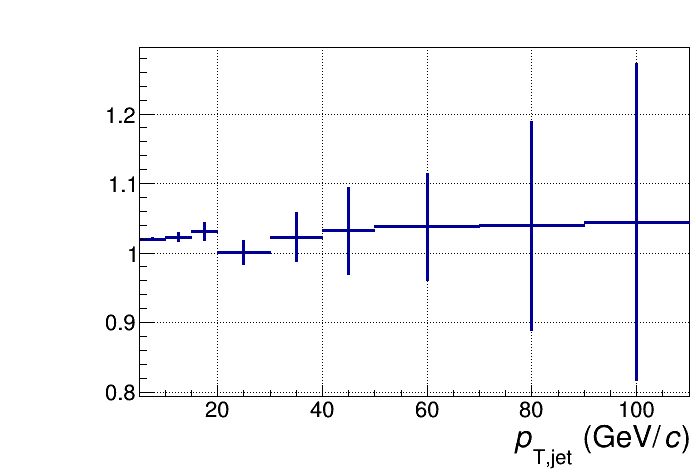
\includegraphics[width=0.40\textwidth]{SysR02_EReso} &
    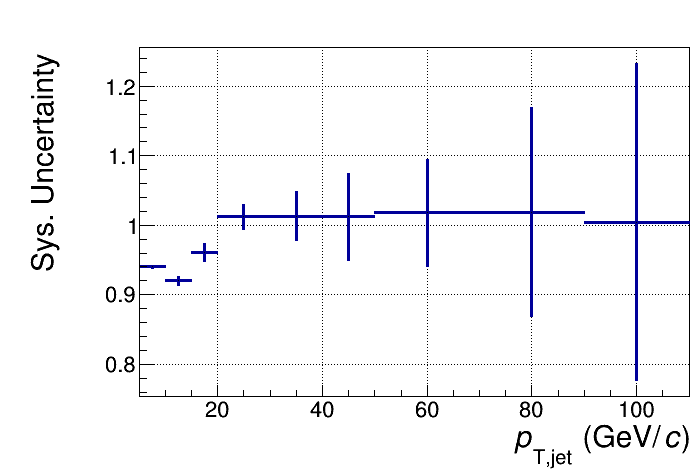
\includegraphics[width=0.40\textwidth]{SysR03_EReso}\\
    \multicolumn{2}{c}{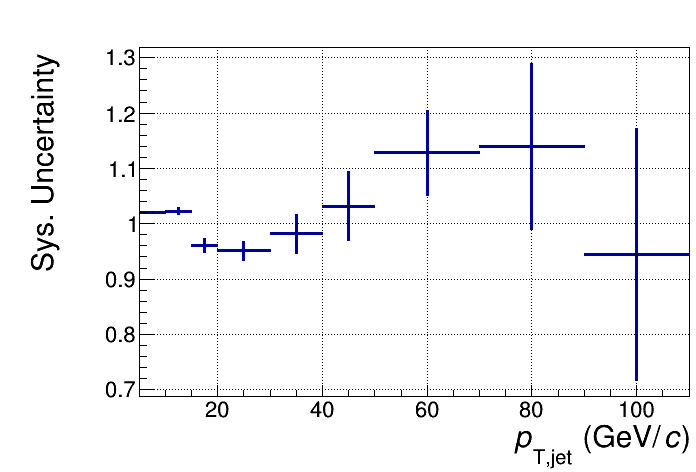
\includegraphics[width=0.40\textwidth]{SysR04_EReso}}
\end{array}$
\caption[Systematic due to energy resolution.]{\label{fig:Eeff}Systematic due to the energy resolution; R = 0.2 \textit{(top left)}, R = 0.3 \textit{(top right)}, R = 0.4 \textit{(bottom)}.}
\end{figure*}

Similar to the $p_{T}$ resolution, the uncertainty due to the EMCal energy resolution is done by smearing the energy of the clusters by the energy resolution function measured from the test beam and seen in Figure \ref{fig:EMCalres}.  The ratio of the spectra with the smear versus the original spectra are show in Figure \ref{fig:Eeff}. The uncertainties for the R = 0.2 and R = 0.3 jets appear well defined and around 1\% - 2\%.  The large variation with R = 0.4 jet energy resolution is due to low statistical fluctuations and a conservative 5\% uncertainty was assigned to this radii.

\subsubsection{Luminosity and Uncertainty}

The luminosity of a hadronic collider, $\mathscr{L}$, is given by the expression



\begin{equation}
\mathscr{L} = \frac{R}{\sigma}
\label{eq:xlumdef}
\end{equation}

\noindent
where R is the interaction rate and $\sigma$ is the visible cross section.  Due to the fact that we only measure events within a 10 cm window within the primary vertex region of ALICE we must scale the total luminosity to that which is delivered within the experiment.  This scale factor is determined by dividing the total number of Min Bias events to those accepted within the 10 cm window.  $N^{tot}_{MB} / N^{10 cm vertex}_{MB}$ = 1.024, which was obtained from the event QA criteria used in this analysis as discussed in Chapter \ref{ch:analysis}.
The total cross-section and luminosity along with there uncertainties were determined during a a special 8 TeV Van der Meer scan run performed in April of 2012\cite{ALICE-PUBLIC-2017-002}.  The total systematic uncertainty for the Min Bias trigger were obtained by measuring the visible cross-section using the T0 and V0 detectors.  The Min Bias trigger was defined as V0AND which required a hit in both the V0A and V0C.  The cross section was reported as being a combined average for Min Bias with the V0AND as, 

\begin{equation}
\sigma_{V0} = (55.8 \pm 1.2) \, mb
\label{eq:xlumdef}
\end{equation}

\noindent
with a combined systematic uncertainty of 2.19\% on the visible cross section and 2.60\% on the luminosity.  Both this cross-section and its uncertainty were scaled by the 1.024 factor to account for the 10 cm vertex region in ALICE before combining with the spectra to obtain the final cross-sections.


\subsubsection{Total Uncertainty}

A summary of the total systematic errors used in the final analysis is given in Table \ref{table:1}.  Some of the uncertainties, for example the $p_{T}$ resolution, used an asymmetric value between the low-$p_{T}$ range, below 40 GeV/\textit{c}, versus high$p_{T}$ range, above 60 GeV/\textit{c}, to account for the statistical fluctuations in the bin filling.  The systematic uncertainties to the yield and JES are added in quadrater together to form the final reported total systematic errors per $p_{T}$ bin.
\newline

\begin{table}[h!]
\centering
\begin{tabular}{ |p{5cm}||p{3cm}|p{3cm}|p{3cm}|  }
 \hline
 \multicolumn{4}{|c|}{Systematic Errors} \\
 \hline
 Systematic &R = 0.2 Jets & R = 0.3 Jets& R = 0.4 Jets\\
 \hline
Clusterization (low-$p_{T}$) & 1.0\%    &1.0\%&  3.0\%\\
 (high-$p_{T}$)           &  5.0\%  & 10.0\%   &  10.0\%\\
Hadronic (all bins)&   5.0\% & 4.0\% & 5.0\%\\
Track Eff (low-$p_{T}$)&20.0\% & 15.0\% & 15.0\%\\
 (high-$p_{T}$)            &  25.0\%  & 20.0\%   &  25.0\%\\
Unfolding (all bins)& 6.0\% & 6.0\%&  6.0\%\\
$p_{T}$ Resolution & 2.0\% & 1.0\% & 4.0\%\\
E Resolution& 2.0\%   &1.0\% & 5.0\%\\
Luminosity (all bins) & 2.2\%  & 2.2 \% & 2.2\%\\
 \hline
 \hline
Total Sys (low-$p_{T}$) & 8.9\%  & 6.6\% & 10.9\%\\
(high-$p_{T}$) & 10.3\%  & 9.1 \% & 14.5\%\\
\hline
\end{tabular}
\caption{Summary of JES and Yield Uncertainties.}
\label{table:1}
\end{table}


\section{8 TeV Inclusive Jet Results and Discussion}

\subsubsection{Differential Jet Cross-Section}

\begin{figure}[h]
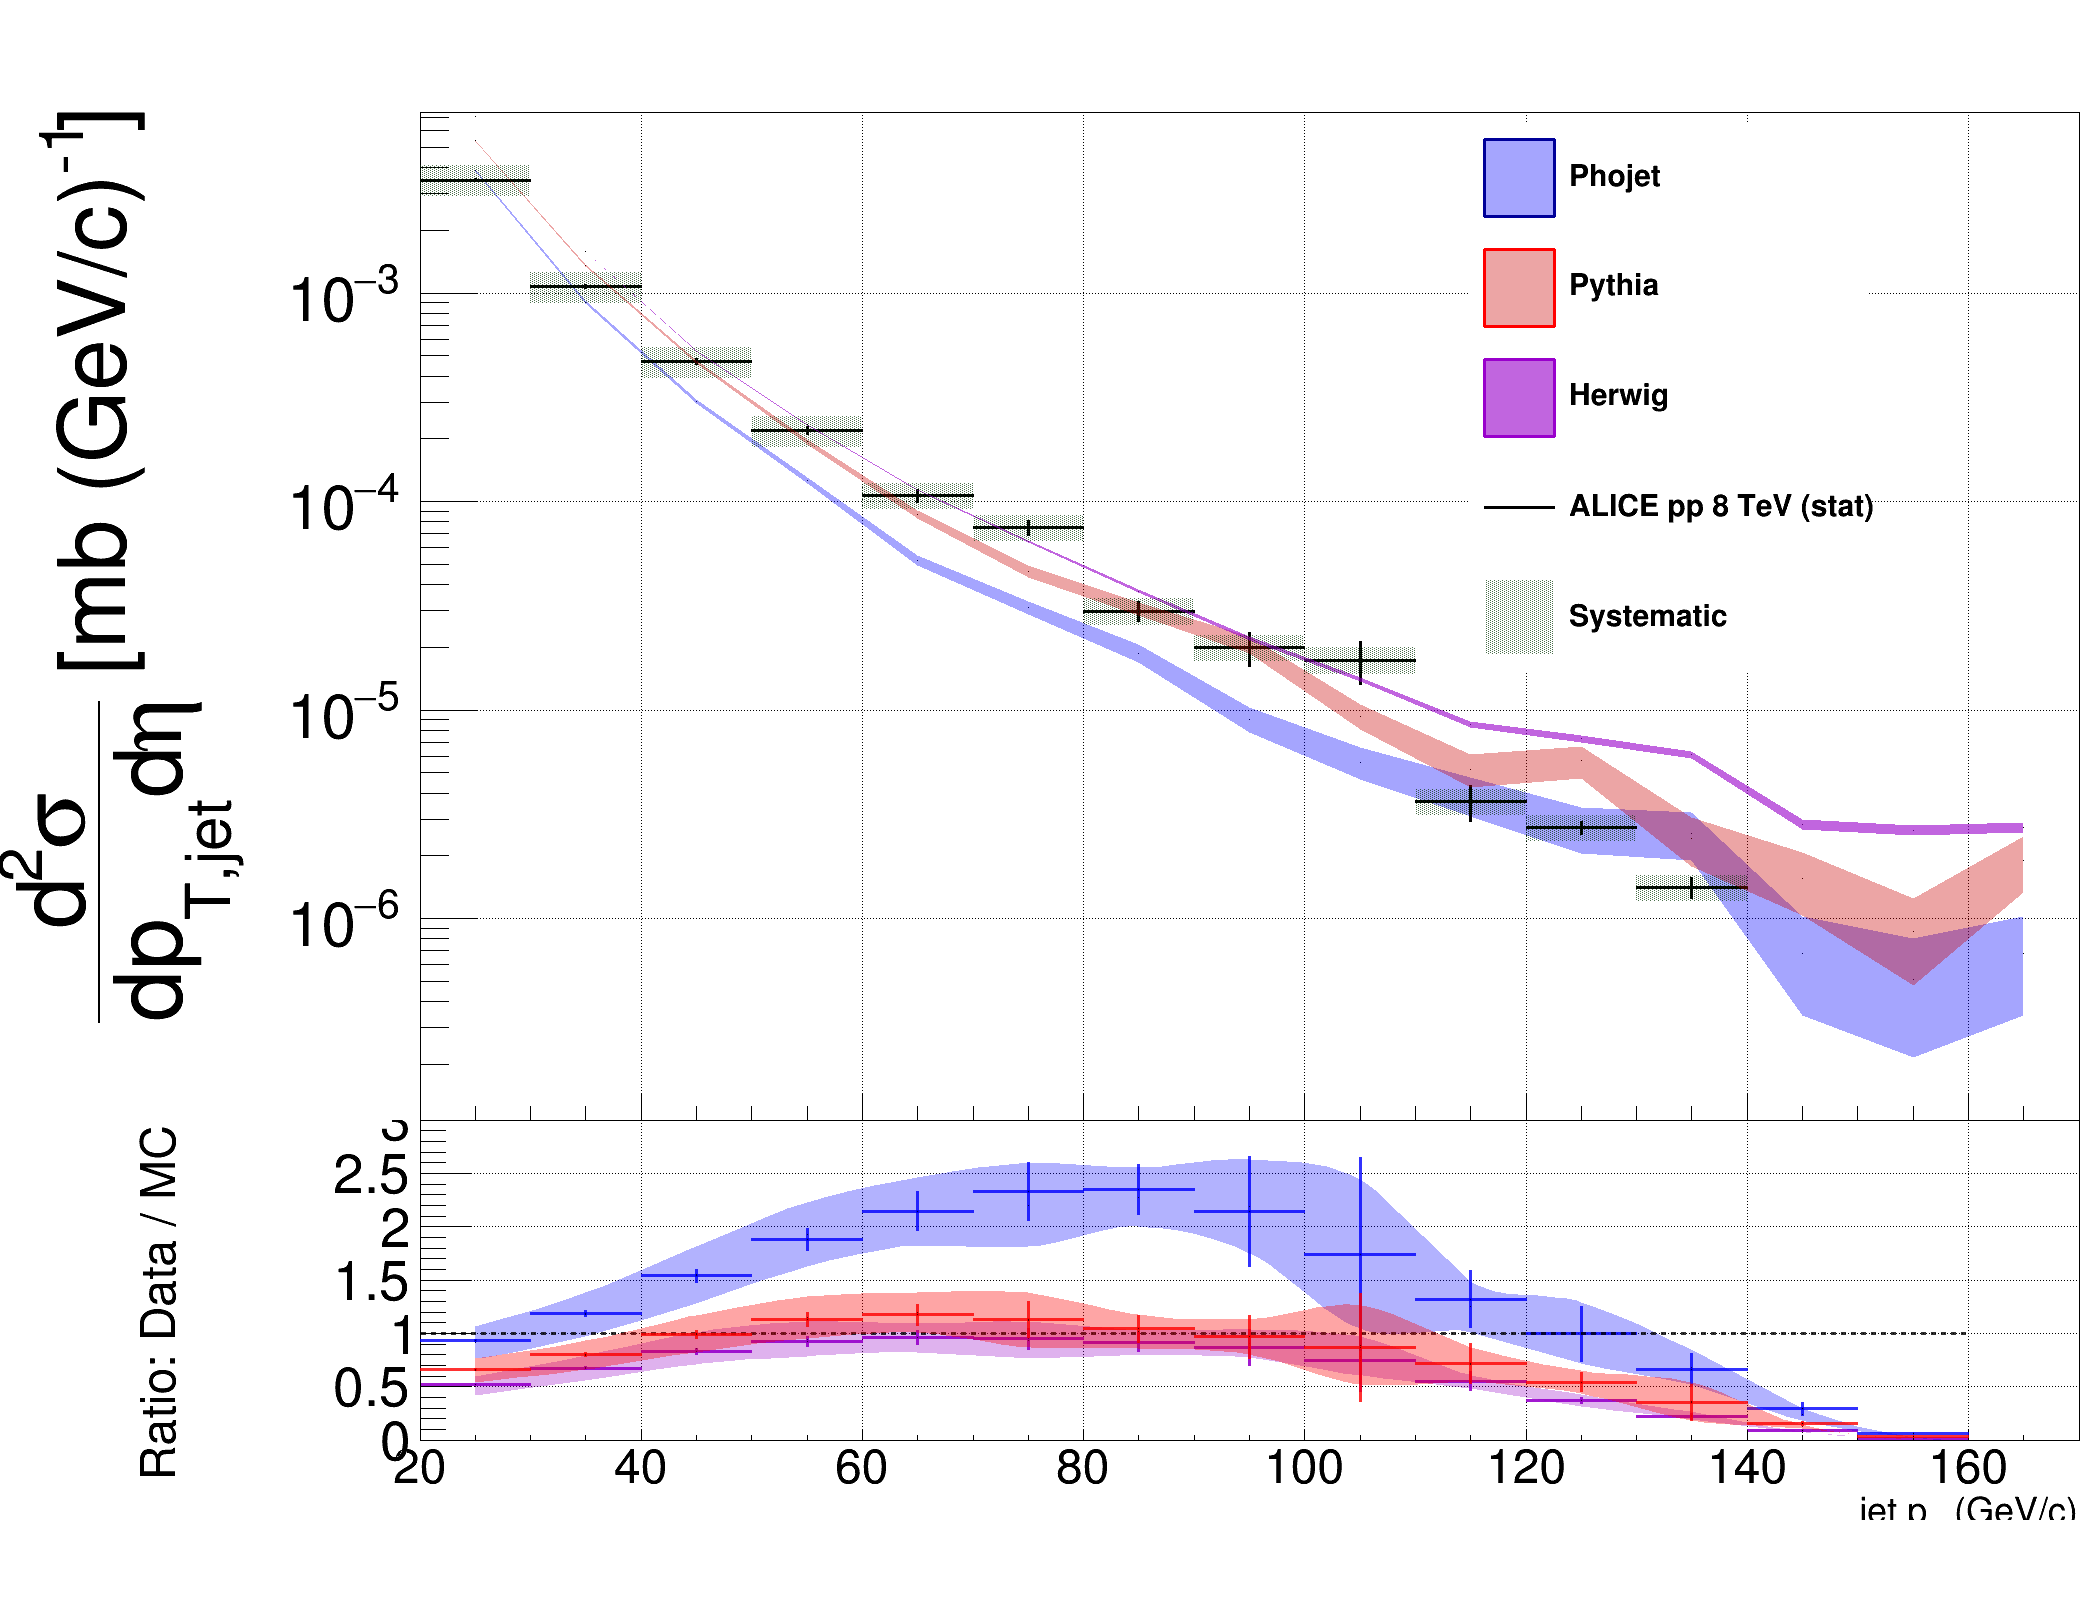
\includegraphics[width=8.5cm]{XSecR02}
\centering
\caption{8 TeV inclusive jet differential cross-section for R = 0.2.}
\label{fig:JetXsecR02}
\end{figure}

\begin{figure}[h]
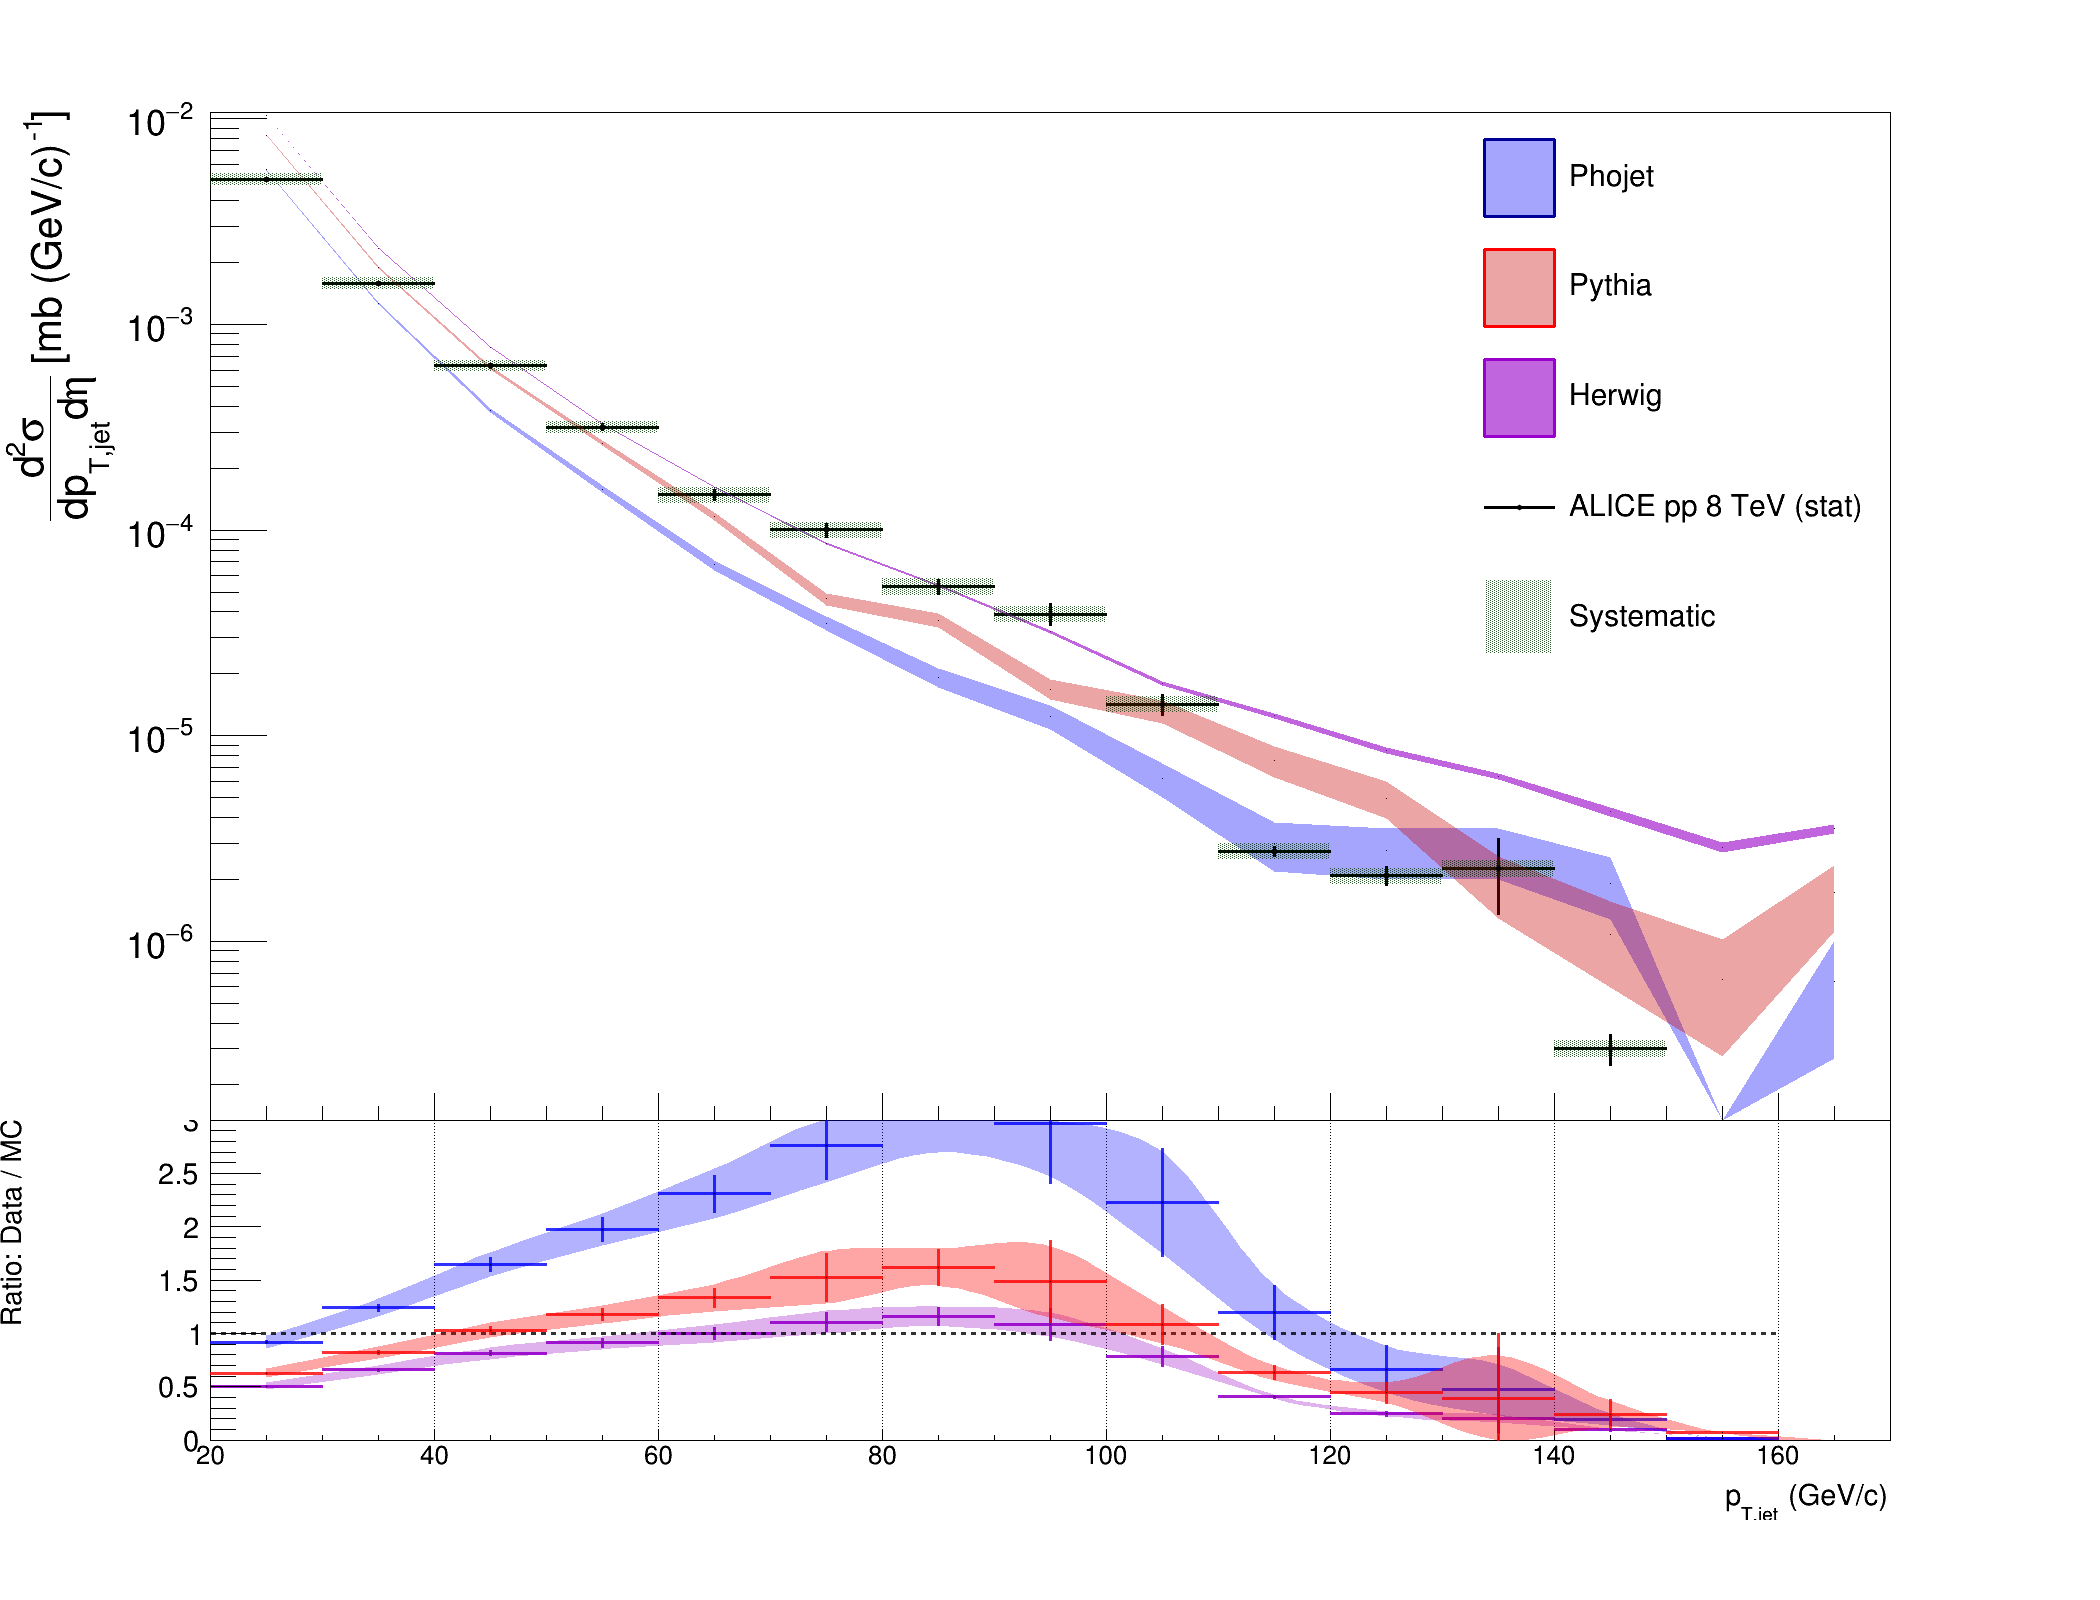
\includegraphics[width=8.5cm]{XSecR03}
\centering
\caption{8 TeV inclusive jet differential cross-section for R = 0.3.}
\label{fig:JetXsecR03}
\end{figure}

\begin{figure}[h]
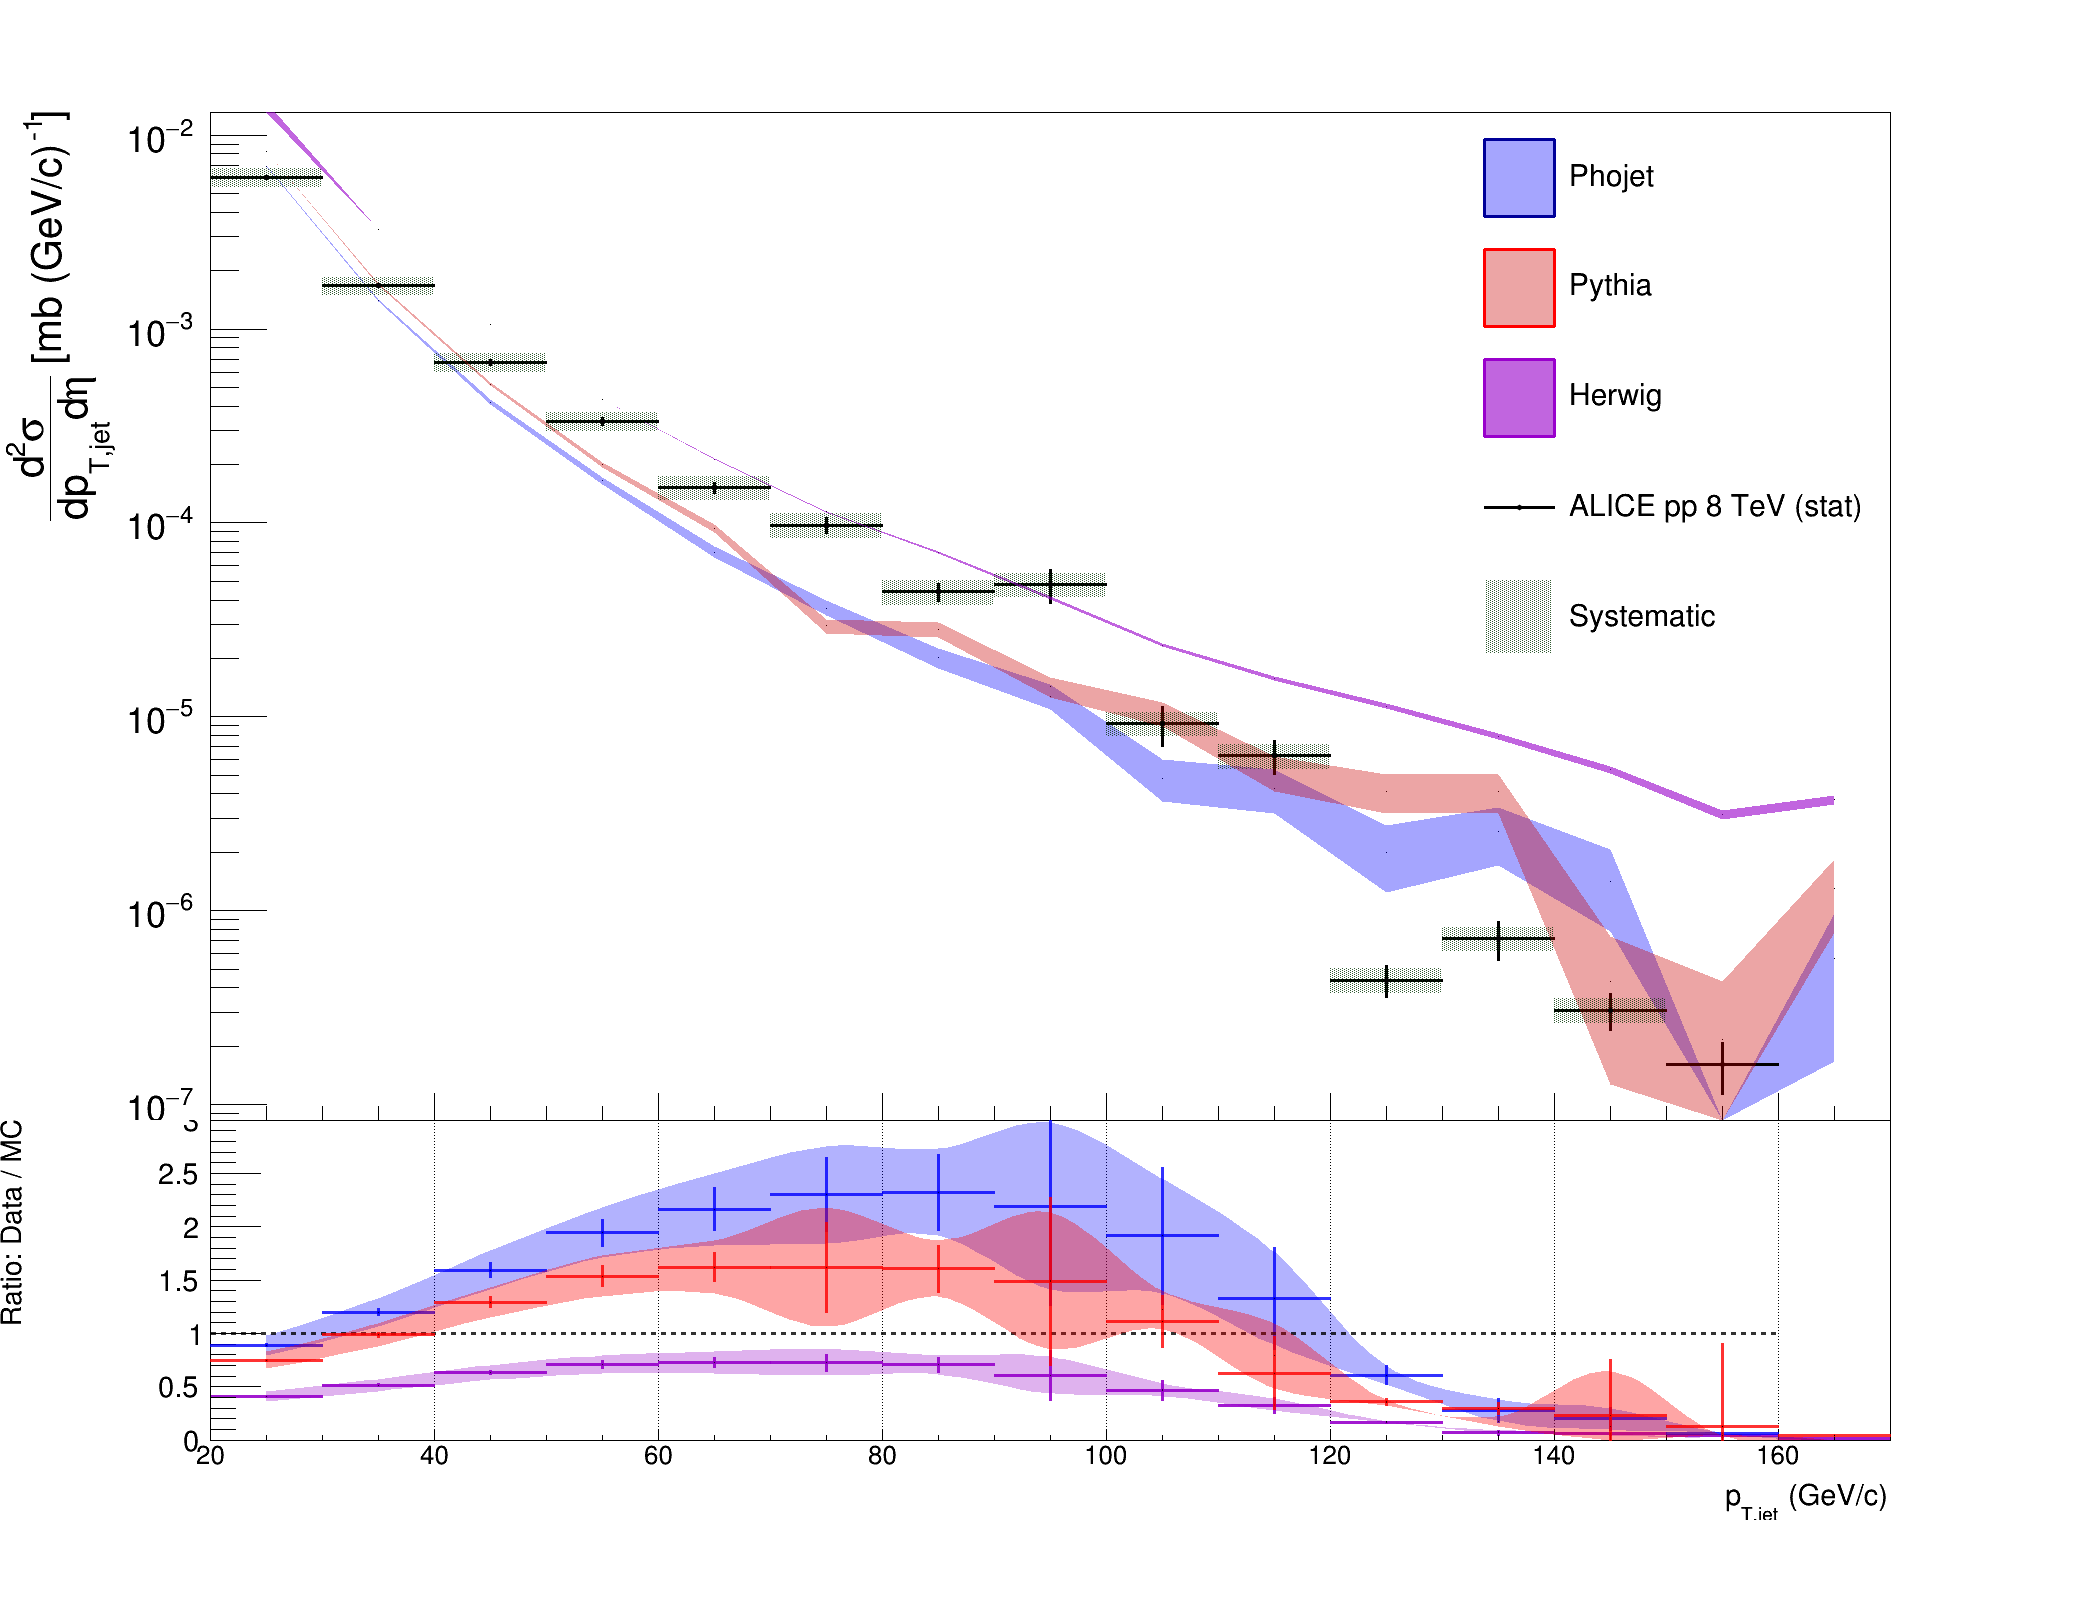
\includegraphics[width=8.5cm]{XSecR04}
\centering
\caption{8 TeV inclusive jet differential cross-section for R = 0.4.}
\label{fig:JetXsecR04}
\end{figure}

\noindent
Figures \ref{fig:JetXsecR02}, \ref{fig:JetXsecR03}, and \ref{fig:JetXsecR04} show the inclusive jet cross-sections from R = 0.2 through R = 0.4 jet radii.  The figures are split into two sections.  The cross-sections as measured from ALICE along with the associated statistical errors are shown in black.  The associated systematic errors from the ALICE data as discussed in this chapter are shown as the green shaded area.  Min Bias Monte Carlo generated events from Pythia (Red), PHOjet (blue), and Herwig (magenta) are included and shown as colored bands to convey the statistical uncertainties from each simulation.  On the bottom half of each plot are the relative ratios of the ALICE jet cross-sections to one of the Monte Carlos using the same color scheme as above.  

What can we tell from these results?  First, we can see that the cross-sections are measured over a wide range, about five orders of magnitude, between 20 GeV/\textit{c} to 160 GeV/\textit{c} in $p_{T}$.  The R = 0.2 and R = 0.3 cross-sections show a well defined trend between 20 GeV/\textit{c} - $\sim$100 GeV/c, after this point the data  has a hard drop after which the data points show wider fluctuations.  This same trend is seen in the R = 0.4 jet cross-section but the jerk happens earlier in $p_{T}$ around  80 GeV/\textit{c}.  The fluctuations are an artifact of the bin-by-bin corrections and the lack of EMCal trigger simulations as discussed in Chapter \ref{ch:analysis}.  

Comparing the data to the Monte Carlos we see that the two simulations produced by the ALICE Collaboration, Pythia and PHOjet, tend to under predict the data.  PHOjet has the least agreement with the data.  The poor agreement with PHOjet can be explained by the fact that PHOjet is an older Monte Carlo generator and better tuned to describing lower energy experiments from the past.  PHOjet may also be under estimating the data because it focuses on describing photon interactions.  The Monte Carlo Simulation from Herwig was produced on a local server farm at the University of Tennessee.  I used a Min Bias tune of Herwig and generated 150 million events and we see that reflected in the low statistical errors.  The Herwig simulation tends to slightly over predict the data.  Both Herwig and Pythia agree well with the data between 20 GeV/c to 100 GeV/c.  It is hard to say that one is `better' then the other because of the relatively large statistical errors from Pythia.  However, for the R = 0.4 jet cross-section we can see that the data seems to trend better towards the clusterization description of hadronization used in Herwig.

Through scaling these results may serve as a reference for heavy-ion collisions and help to better constrain our understanding of parton energy loss mechanisms in the QGP.  


\subsubsection{Jet Cross-Section Ratios}

\begin{figure}[h]
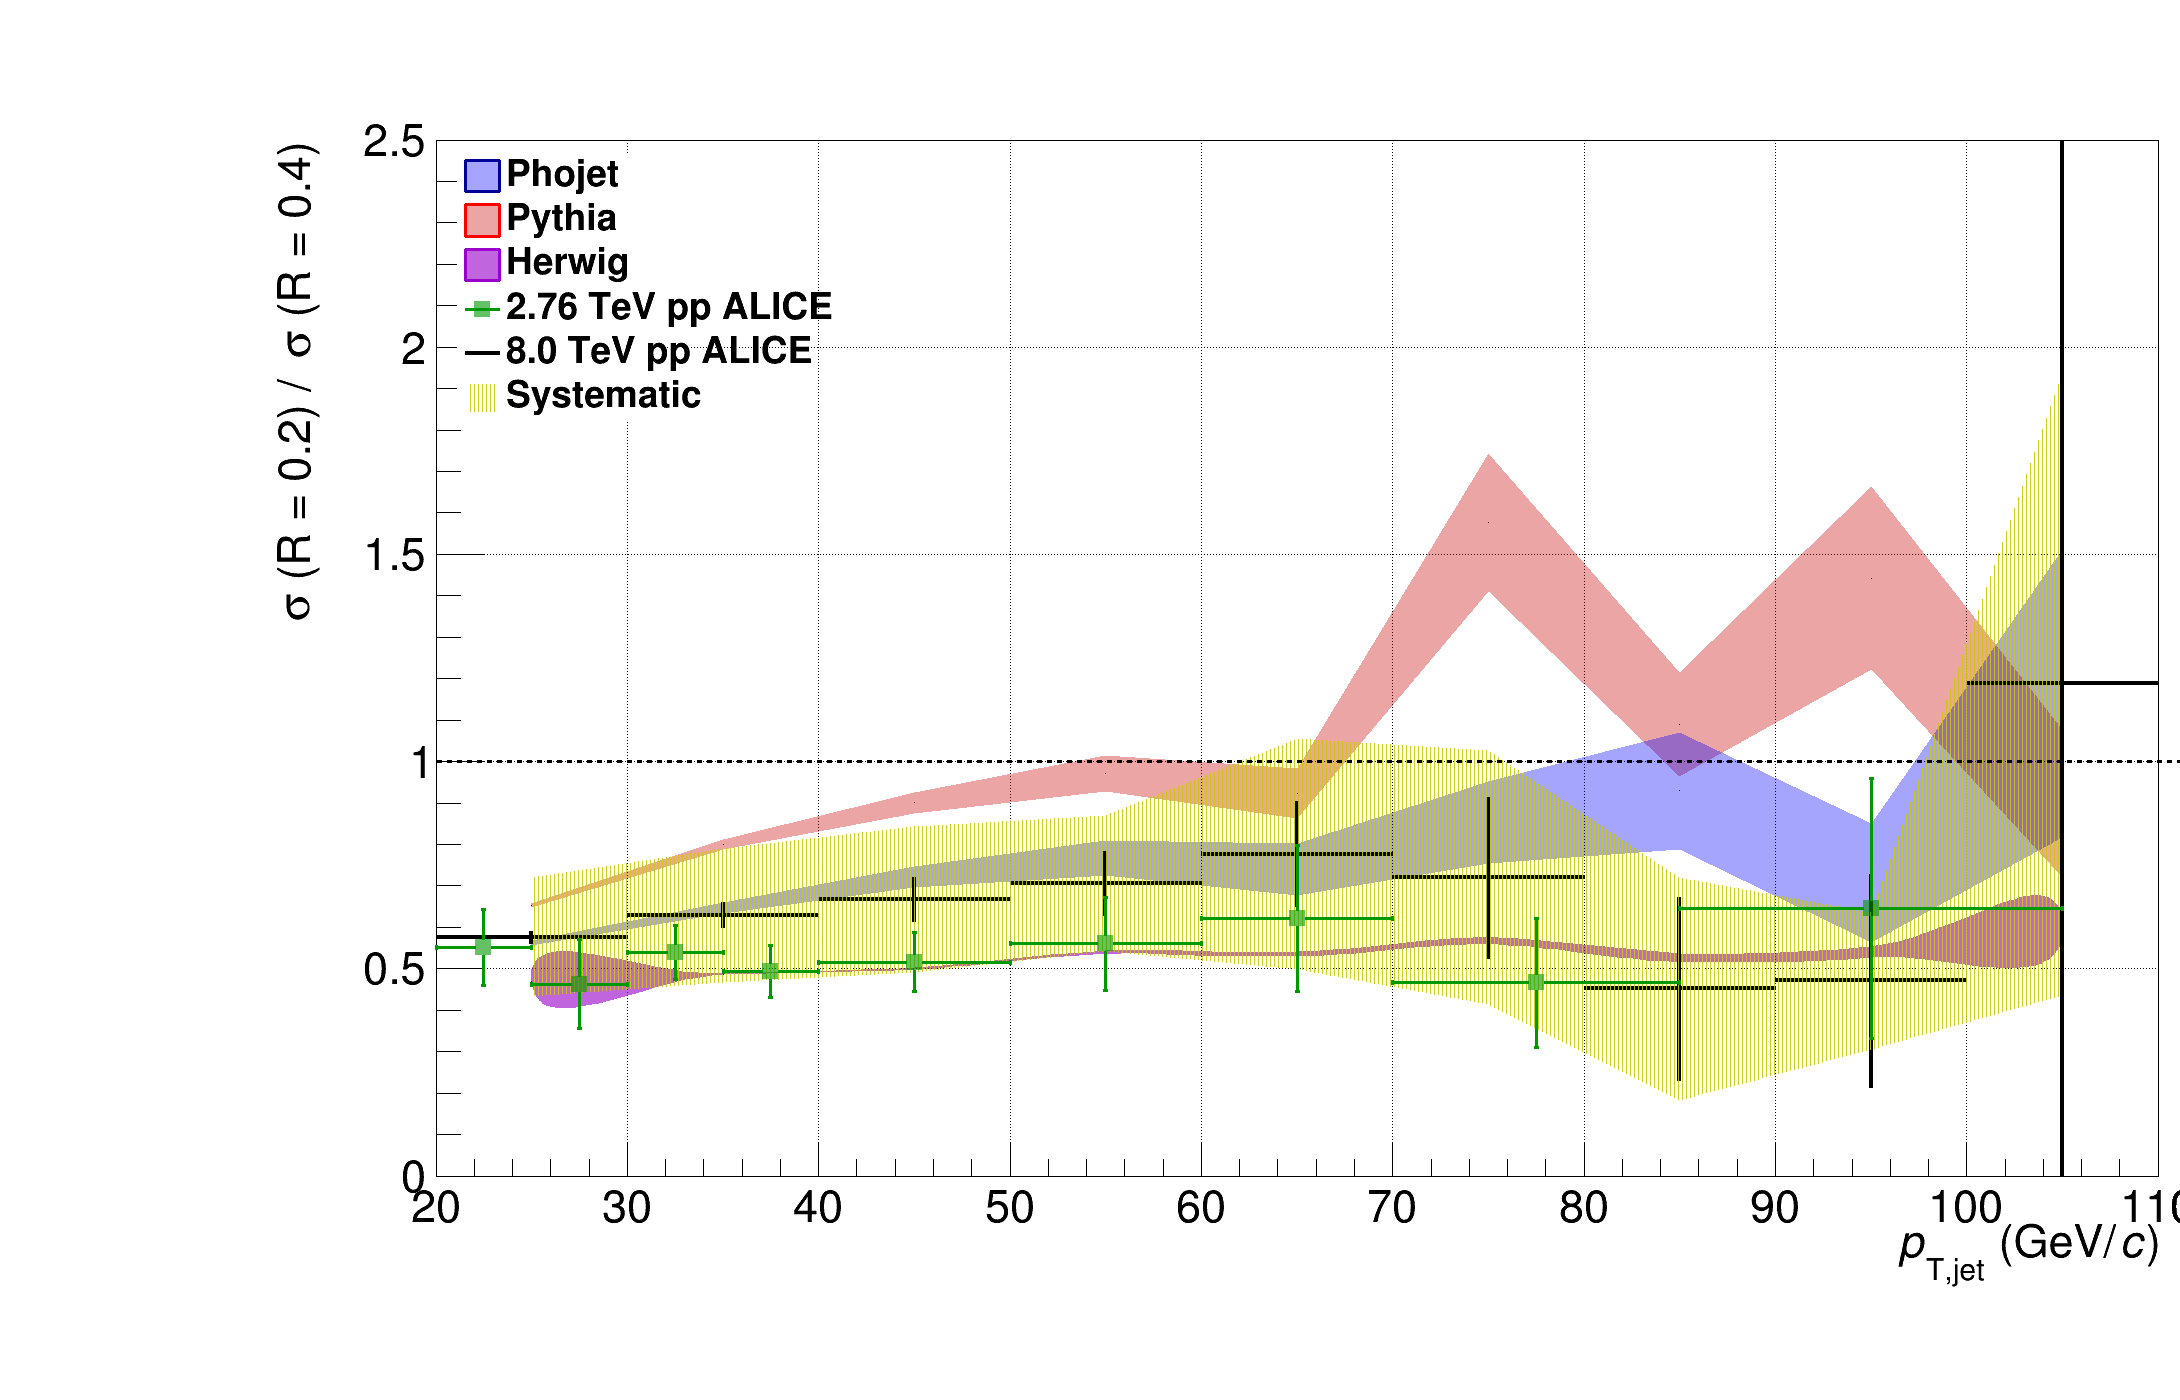
\includegraphics[width=8.5cm]{XSecRatioR02}
\centering
\caption{Ratio of the jet cross-sections R = 0.2  to R = 0.4.}
\label{fig:JetXsecRatioR02}
\end{figure}

\begin{figure}[h]
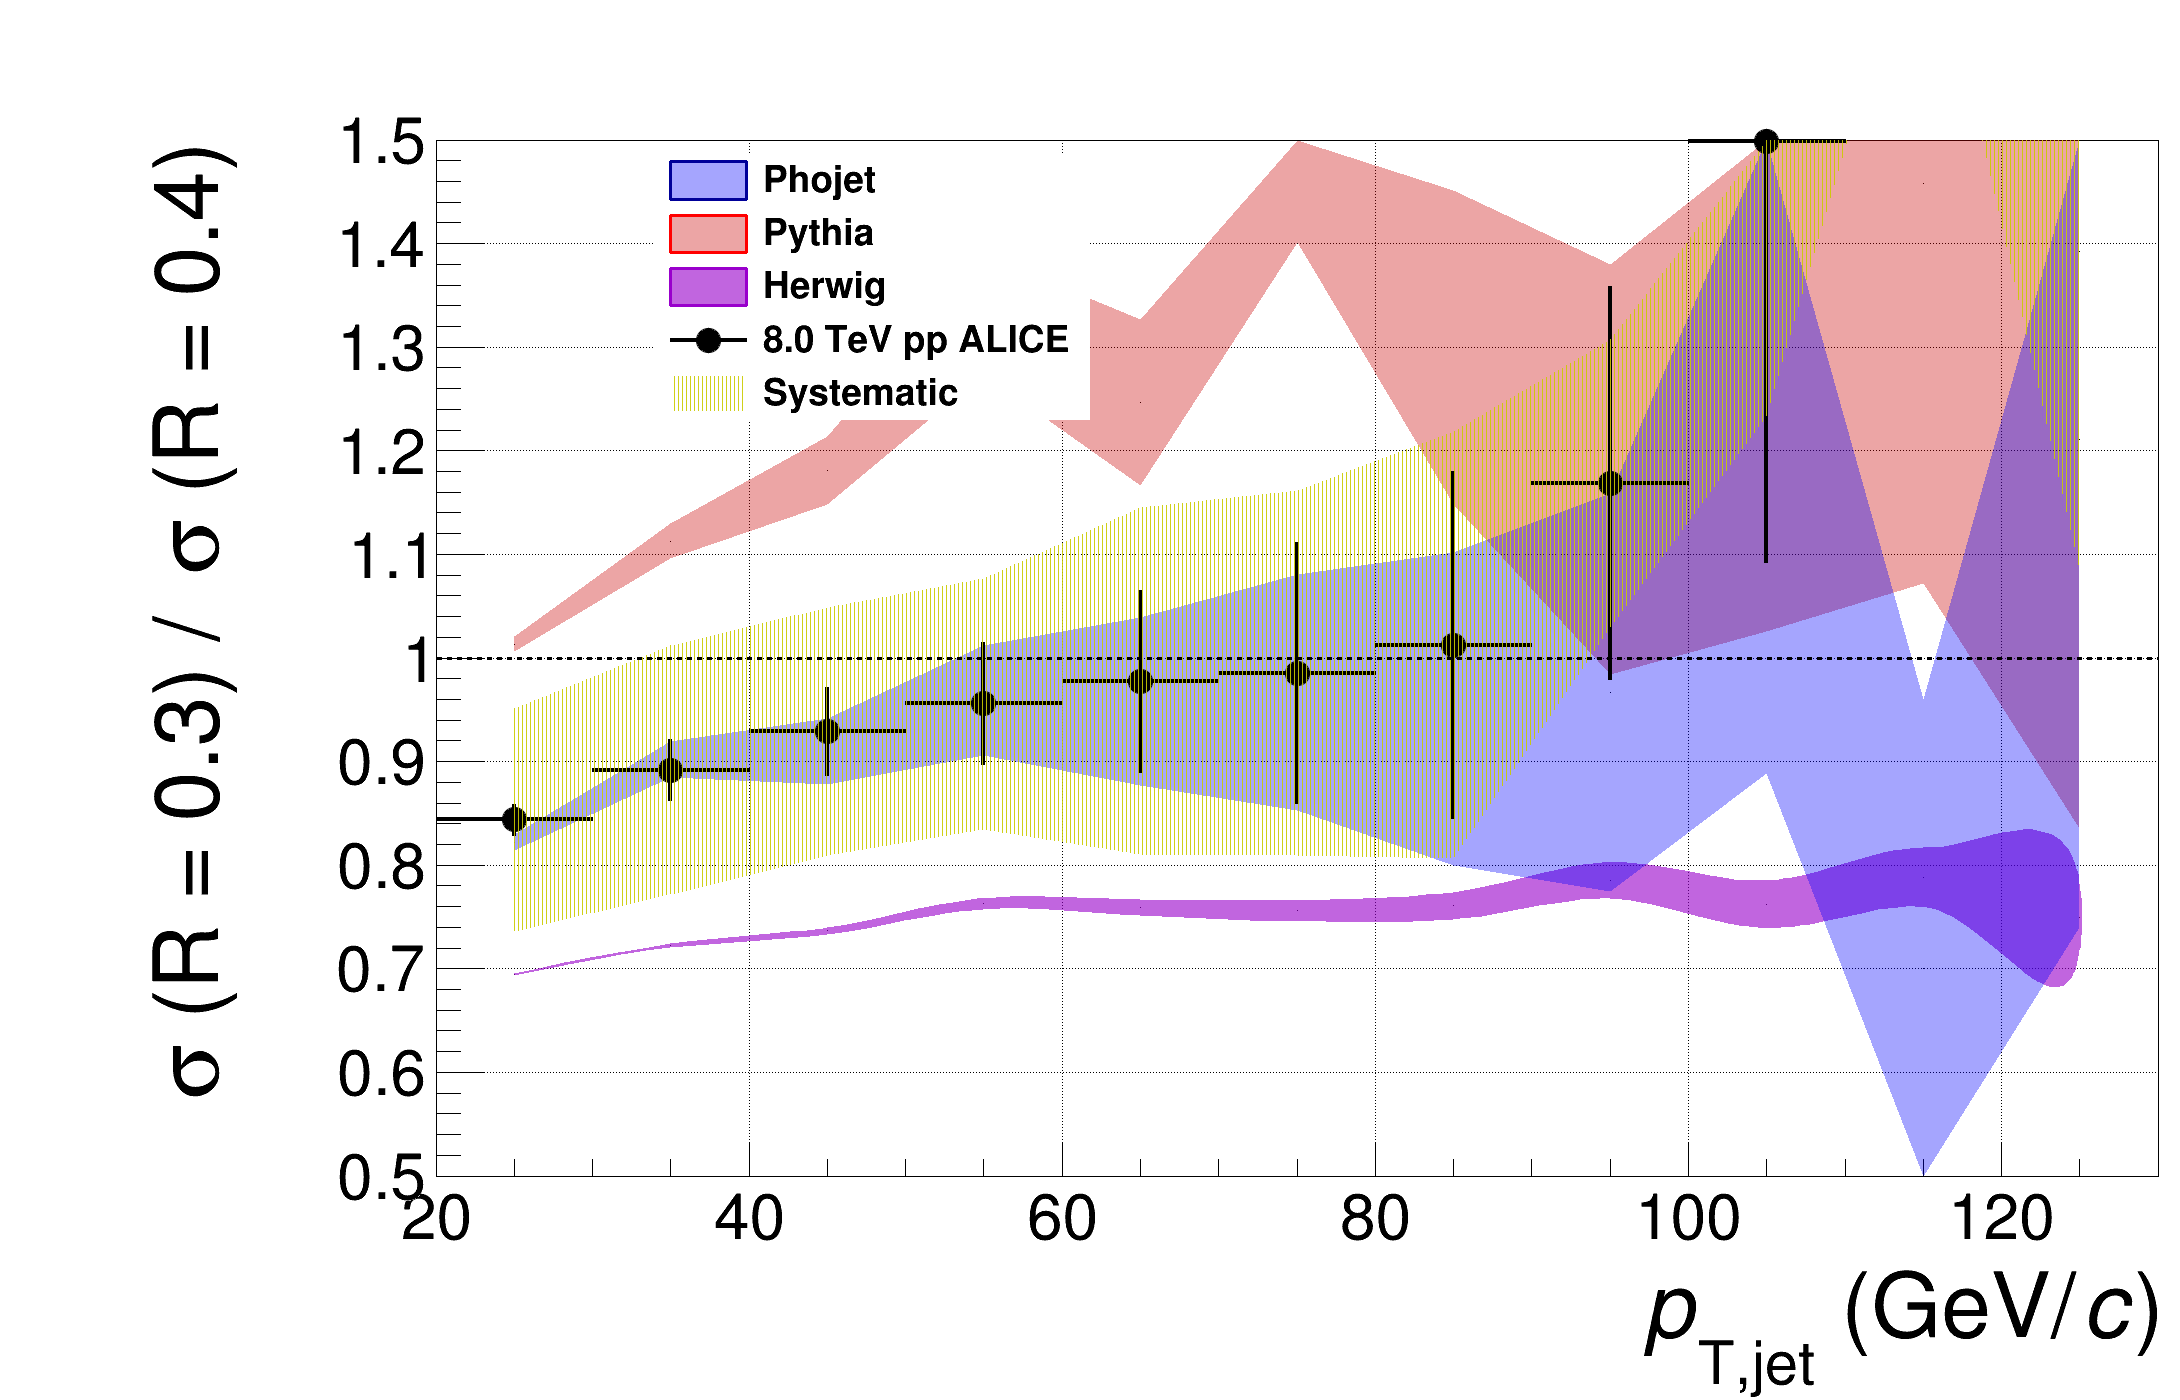
\includegraphics[width=8.5cm]{XSecRatioR03}
\centering
\caption{Ratio of the jet cross-sections R = 0.3  to R = 0.4.}
\label{fig:JetXsecRatioR03}
\end{figure}


\begin{figure}[h]
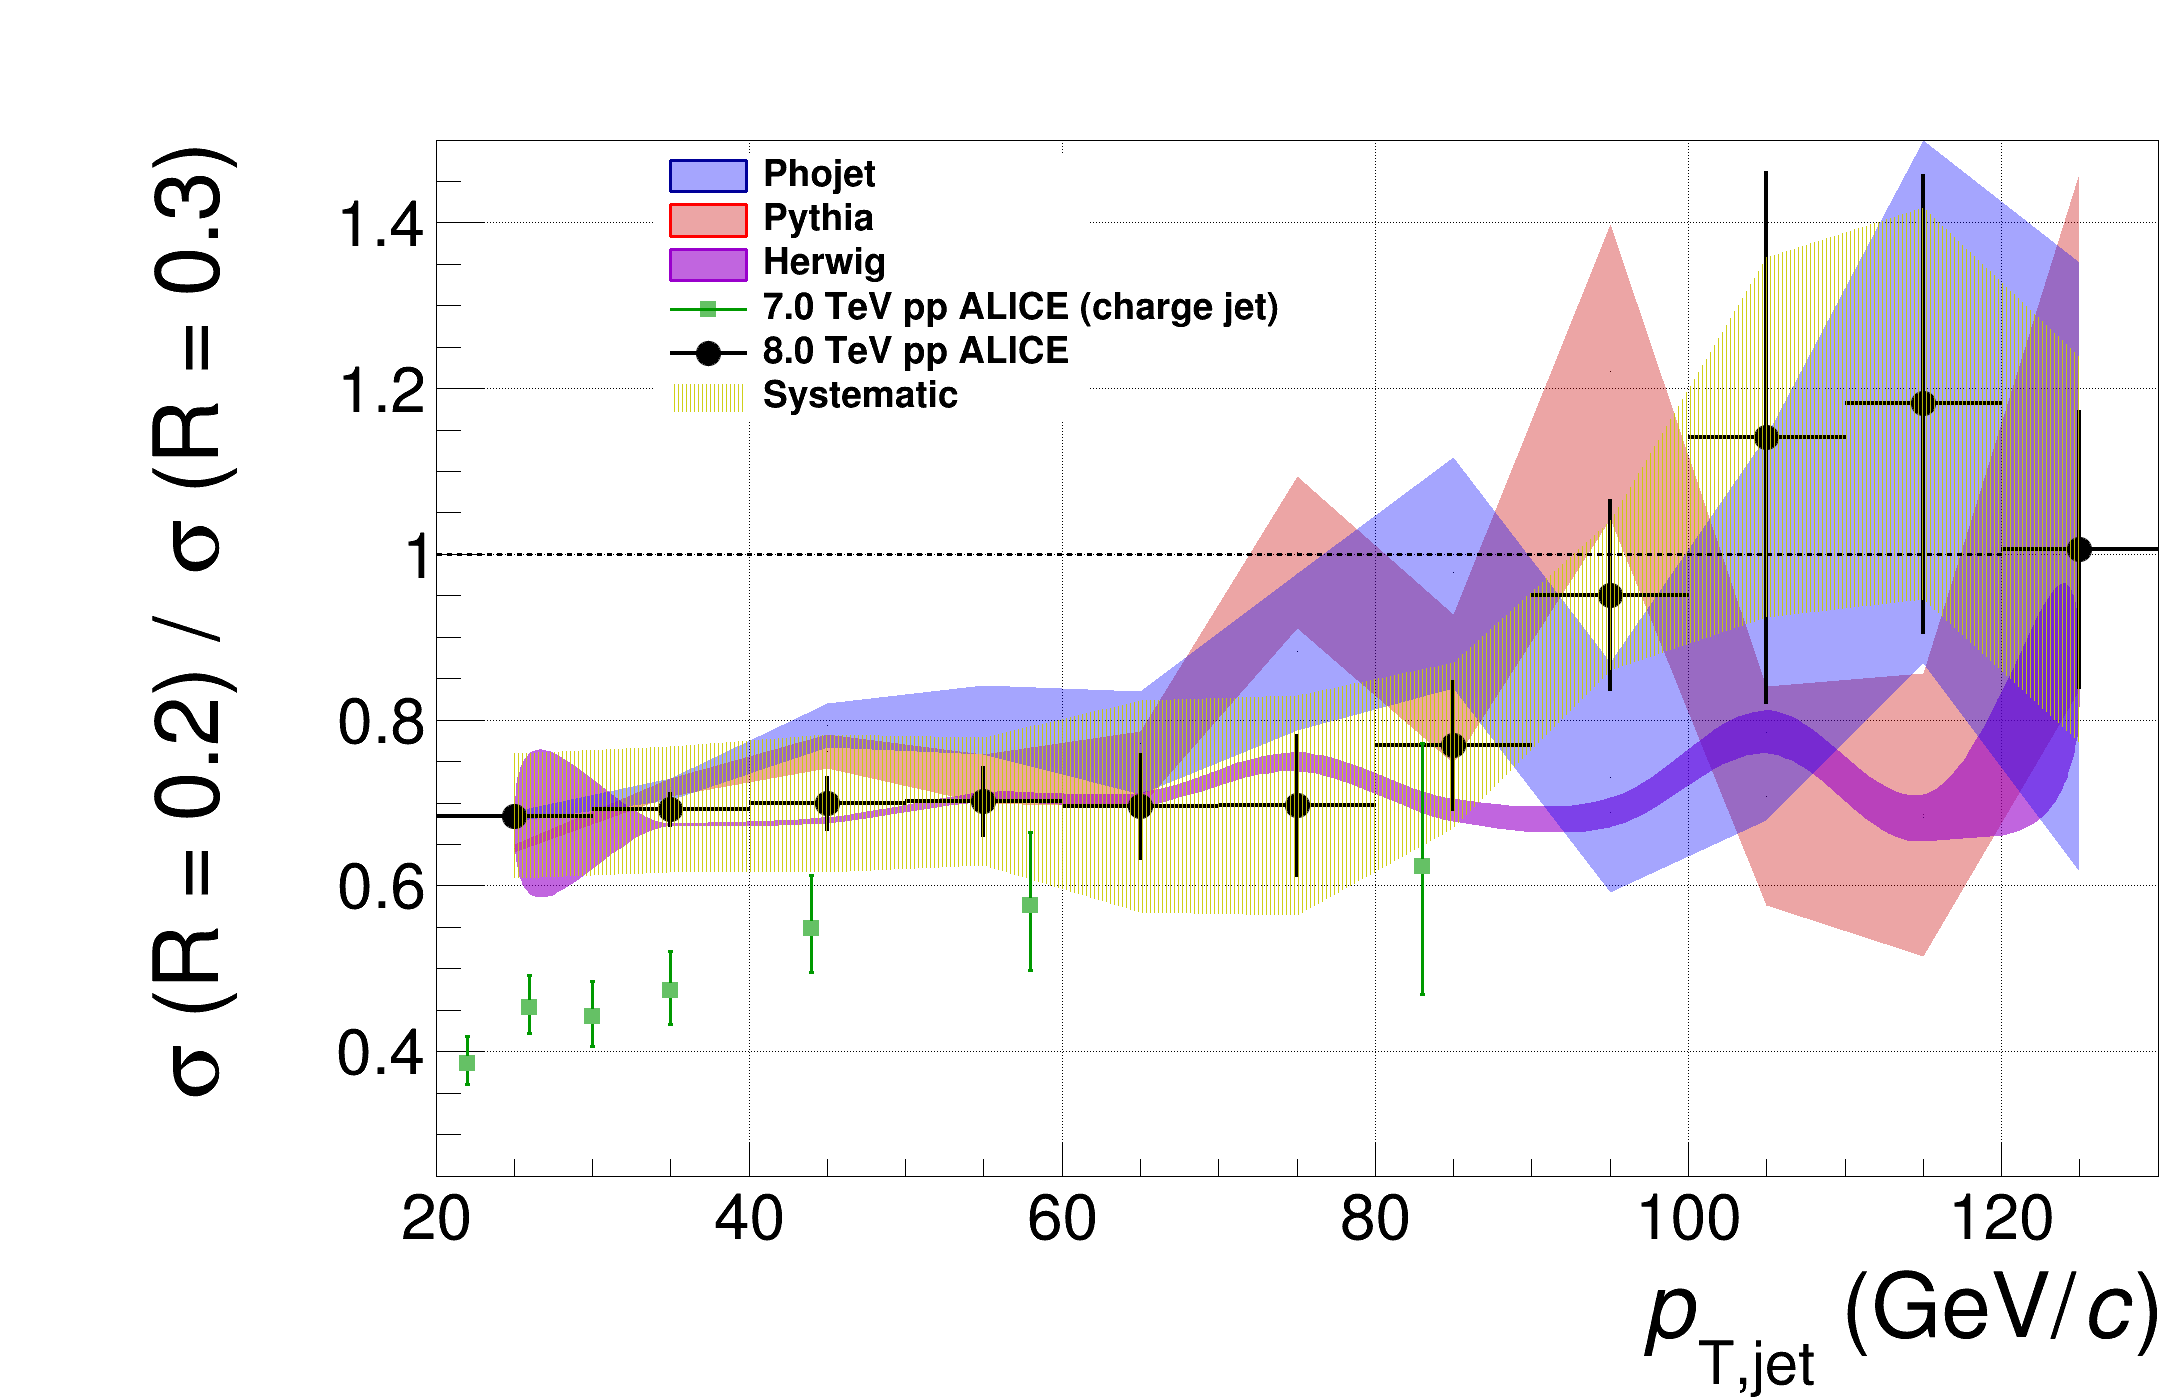
\includegraphics[width=8.5cm]{XSecRatioR023}
\centering
\caption{Ratio of the jet cross-sections R = 0.2  to R = 0.3.}
\label{fig:JetXsecRatioR023}
\end{figure}


\noindent
The ratio of the jet cross-sections as a function of the jet radii is defined as,

\begin{equation}
\mathscr{R} (p_{T}; \, R_{1},R_{2}) = \frac{d\sigma(R_{1}) /d\eta \, dp_{T} }{d\sigma (R_{2}) /d\eta \, dp_{T}},
\label{eq:jetxsecratio}
\end{equation}

\noindent
where $R_{1}$ and $R_{2}$ are the jet radii in question. This probes the transverse structure of jets and is sensitive to QCD hardonization\cite{SOYEZ201159}.  Figures \ref{fig:JetXsecRatioR02}, \ref{fig:JetXsecRatioR03}, and \ref{fig:JetXsecRatioR023} report the ratios of the jet cross-sections between R = 0.2 / R = 0.4, R = 0.3 / R= 0.4, and R = 0.2 / R = 0.3 respectively.  The figures also show the relative ratios plotted from the 8 TeV ALICE data, Pythia, PHOjet, and Herwig using the same color schema as the jet cross-sections.  Errors between the cross-sections of different radii are considered uncorrelated and added in quadrature to form the error bars reported in the figures.

A similar analysis to this thesis was performed using a 2.76 TeV  data sample collected from ALICE\cite{MA2013319} and it is compared to Figure \ref{fig:JetXsecRatioR02} and \ref{fig:JetXsecRatioR023} in green bullet points.  In order to avoid double counting by sampling the same jet  found using an R = 0.2 and R = 0.4 jet finder these ratios use disjointed samples of the 8 TeV data set.  From the results of the cross-section ratios, we see that the 8 TeV data as reported from this thesis agrees well with the 2.76 TeV results in Figure \ref{fig:JetXsecRatioR02}.  Interestingly it seems that the PHOjet Monte Carlo agrees well with the data for all three figures and is the simulation that agrees the best for the $\sigma (R = 0.3)$ / $\sigma (R = 0.4)$ ratio.  It can be concluded that the Pythia ratios have the least agreement because it only includes the LO matrix to calculate partonic showers, which does not model the angular ordering of QCD radiation very well.  Herwig tends to under predict the data, especially at low-$p_{T}$, which is expected and may be understood in terms of limitations modeling low energy background particles with tune used in this thesis (v2.3).  

Similar to the previous results these ratios can be used to constrain jet quenching in the QGP.  These results also report the first ratio of jet cross-sections between R = 0.2 and R = 0.3.  This is especially helpful for heavy-ion collisions as most jet results from heavy-ions use either an R = 0.2 or R = 0.3 jet radius to suppress the background in the high multiplicity environment.


\section{Conclusion}

Jet cross-sections are a result of QCD interactions while the ratios of the cross-sections for jets of different radii probe the hadronization process.  The essential nature of how hadronization effects the jet cross-sections is still an open question and should be probed in future measurements at the LHC.  ALICE is in the unique position of being able to reconstruct full jets over a wide kinematic range, especially to low momentum.

This thesis presents the first measurements of inclusive full jets at $\sqrt{s} = \,$ 8 TeV using the ALICE detector.  It also presents a procedure, by which using a set of corrections and QA criteria, we may obtain results comparable to pQCD Monte Carlo simulations.  The agreement between the results and Monte Carlo simulations show the jets are a well calibrated probe for testing QCD phenomena.  In terms of the kinematic reach, the results of this thesis are in good agreement with QCD calculations down to 20 GeV/\textit{c} through 100 GeV/\textit{c} in $p_{T}$.  This range may be extended with better Monte Carlos in the furture and this is currently being worked on until the results are published.  With a better Monte Carlo production we could see the range extend to between 5 GeV/\textit{c} to about 200 GeV/\textit{c} in $p_{T}$.  The comparisons with the Monte Carlos agree well, with the most tension lying with PHOJET.  However, these results are expected to improve once an improved GEANT4 Monte Carlo that models the EMCal trigger is made available.  

It is striking how well both hadronization models, the Lund-String model and Clusterization model encompassed by Pythia and Herwig, agree with the data.  These are fundamentally different physics phenomenology and it begs the question , why this is?   It is interesting and exciting that some of the initial questions posed when I started my Ph.D. work remain and I am hopefully for new insights from future work in both theory and experiment.  

The results from this thesis can also be used in future heavy-ion runs to probe jet quenching, as these results would serve as a baseline comparison.  The work in this thesis also presents the jet measurements from ALICE down to 20 GeV/\textit{c}, which will be important for probing energy loss in the QGP.  By measuring these very low energy jets we can probe the full energy loss mechanism for partons traversing the QGP.  Previous higher energy jet results would tend to bias to jets that traveled a very short distance through the QGP.

With the increase in energy and luminosity seen at the LHC, we have moved into the era of high-precision testing of pQCD.  The work set forward by this thesis sets the stage for using jets in the future at CERN, especially after the high luminosity upgrade of the LHC is complete.  Although it dates to 2012, the 8 TeV contains some of the largest data sets available at a given energy from the LHC.  This makes it an important data set and worthy of future investigations.  I'm proud of the work presented in this body, both in terms of the data analysis and engineering aspect.  What results we will gain from the upgraded LHC and jets is only left to our imagination and to nature's mercy.